% =====================================================================
%  §9. Идентифицируемость: Фишер, вырождение, профиль, бутстрап
%
%  ЖАНР (STYLE.md): учебная литература. Ни путей, ни имён программ, ни
%  номеров гипотез. Прослеживаемость — ключи \srckey{9.x} и приложение.
%
%  Содержательная основа: BRIEF_FOR_D_teaching_ladder.md §1, §8;
%  SYNTHESIS.md §3, §8.
% =====================================================================
\section{Идентифицируемость: вырождение, профиль, бутстрап}
\label{sec:identifiability}
\markboth{§\thesection. Идентифицируемость}{}

§5 показал на линейной задаче: если два столбца матрицы плана почти коллинеарны, соответствующие
параметры почти неразличимы, и это видно на эллипсе ковариации напрямую. §7 упомянул, что для
нелинейной модели та же болезнь существует, только матрица плана заменяется якобианом в точке
минимума, а эллипс~--- уже не рисуется одной формулой. Здесь этот обещанный переход выполняется до
конца: вводится формальный аппарат (информация Фишера), разбирается конкретное, самое
чувствительное вырождение опорной модели курса, и показывается, почему в вырожденном случае
привычная параболическая оценка ошибки откровенно врёт.

\begin{tcolorbox}[enhanced,colback=cPanel,colframe=cGrid,boxrule=0.8pt,arc=2pt,
                  title={\bfseries\color{cAccent} Пререквизиты},coltitle=cAccent,
                  attach boxed title to top left={xshift=6pt,yshift=-2pt},
                  boxed title style={colback=cPanel,boxrule=0pt,arc=0pt},top=10pt]
\textbf{Нужно знать:} §5 целиком (обусловленность, эллипс ковариации); §7 (целевая функция,
фиксация параметров, бутстрап); §8 (правдоподобие, $\AIC$).\\[0.3em]
\textbf{Знать НЕ нужно:} общую байесовскую теорию идентифицируемости моделей~--- здесь всё
разбирается на одном конкретном, уже знакомом курсу примере.
\end{tcolorbox}

% ---------------------------------------------------------------------
\subsection{Информация Фишера: якобиан вместо матрицы плана}
\label{subsec:fisher}

\begin{strict}
Вблизи максимума правдоподобия (минимума $\chi^2$) логарифм правдоподобия хорошо приближается
параболой, и \term{матрица информации Фишера} играет роль, которую в §5 играла $X^{\mathsf T}WX$:
\begin{equation}
  \mathcal{I}(\mathbf{p}^\star)\approx J^{\mathsf T}WJ,
  \qquad
  J_{i\alpha}=\frac{\partial f(\mathbf{p};x_i)}{\partial p_\alpha}\bigg|_{\mathbf{p}^\star},
  \qquad
  \operatorname{Cov}(\mathbf{p}^\star)\approx\mathcal{I}^{-1} .
  \label{eq:fisher}
\end{equation}
Это тот же самый алгоритм Гаусса--Ньютона, что стоит внутри Левенберга--Марквардта (§7): якобиан
$J$~--- линеаризация нелинейной модели \emph{в точке минимума}. Вся геометрия §5 (эллипсы,
обусловленность, почти коллинеарные столбцы) переносится сюда без изменений~--- меняется только
то, что раньше $X$ была задана планом заранее, а теперь $J$ вычисляется в конкретной, уже
найденной точке и, вообще говоря, меняется от точки к точке.
\end{strict}

\begin{intuition}[: что означают собственные числа $\mathcal{I}$]
Разложение $\mathcal{I}$ по собственным векторам делит пространство параметров на
\term{хорошо определённые} направления (большое собственное число~--- узкое направление
эллипсоида, данные сильно ограничивают соответствующую комбинацию параметров) и
\term{плохо определённые} (маленькое собственное число~--- широкое направление, вдоль него данные
почти ничего не говорят). Как правило, эти направления~--- не отдельные параметры модели, а их
\emph{комбинации}: данные хорошо знают одну линейную (или нелинейную) смесь параметров и почти
ничего не знают об ортогональной ей смеси.
\end{intuition}

% ---------------------------------------------------------------------
\subsection{Конкретное вырождение опорной модели}
\label{subsec:degeneracy}

Самое чувствительное направление опорной модели курса связывает три параметра: эффективный
диаметр $\Deff$ (§\ref{sec:electrodynamics}, §6), амплитуду просачивания~$\eta_0$ (§1, §6) и
перекрёстный член~$\varepsilon_{\rm cross}$ (§6).

\begin{example}[: насколько сильно вырождены $\Deff$ и $\eta_0$]\srckey{9.1}
Корреляция оценок $\Deff$ и~$\eta_0$ при их совместной свободной подгонке составляет
$-0{,}999999$~--- по сути, минус единица. Соответствующая пара параметров ведёт себя не как два
независимых числа, а как одна степень свободы: данные знают некоторую их комбинацию (условно,
<<общий дефицит канала подавления>>) практически точно, а способ, которым эта комбинация делится
между <<геометрией>> и <<просачиванием>>,~--- почти произвольно.
\end{example}

\begin{warning}[: что происходит, если подгонять оба параметра свободно]\srckey{9.2}
Свободная совместная подгонка $\Deff$ на плотной решётке даёт $1{,}85\pm8{,}37$~мкм. Формально
это число с оценкой ошибки; по существу~--- признание того, что данные почти ничего не говорят об
этом параметре по отдельности, замаскированное под результат измерения. Ошибка $8{,}37$~мкм
превышает само центральное значение более чем вчетверо~--- уже этого достаточно, чтобы
заподозрить вырождение прежде, чем разбираться в его происхождении.
\end{warning}

% ---------------------------------------------------------------------
\subsection{Профильное правдоподобие: когда параболическая ошибка врёт}
\label{subsec:profile}

Оценка ошибки из формулы~\eqref{eq:fisher} предполагает, что $\chi^2$ вблизи минимума~---
парабола. Это предположение стоит проверять, а не принимать по умолчанию~--- особенно рядом с
вырождением. \term{Профильное правдоподобие} строится так: параметр (здесь~--- $\Deff$)
поочерёдно фиксируется на серии значений, а на каждом шаге \emph{все остальные} параметры
подгоняются заново. Получается кривая «лучший $\chi^2$ (или $\AIC$) при данном фиксированном
значении $\Deff$» — честная картина того, что данные на самом деле знают об этом параметре, без
предположения о параболичности.

\begin{example}[: профиль не параболичен и не совпадает со свободной оценкой]\srckey{9.3}
Профиль $\AIC(\Deff)$ на плотной решётке имеет глобальный минимум около $\Deff\approx6$~мкм~---
заметно отличается от свободной оценки $1{,}85$~мкм из §\ref{subsec:degeneracy}, и по пути к нему
$\AIC$ ведёт себя не монотонно: есть промежуточные локальные минимумы разной глубины, а не одна
гладкая парабола. Мера «уплощённости» профиля (отношение размаха $\AIC$ на профиле к его
типичному шагу) далека от той, что была бы у чистой параболы. Свободная нелинейная подгонка,
предоставленная себе, не обязана найти этот более глубокий минимум~--- в этом состоит прямая связь
с многостартовой оптимизацией §7: то же самое вырождение, которое портит параболическую оценку
ошибки, одновременно создаёт дополнительные локальные минимумы для алгоритма подгонки.
\end{example}

\begin{figure}[t]
  \centering
  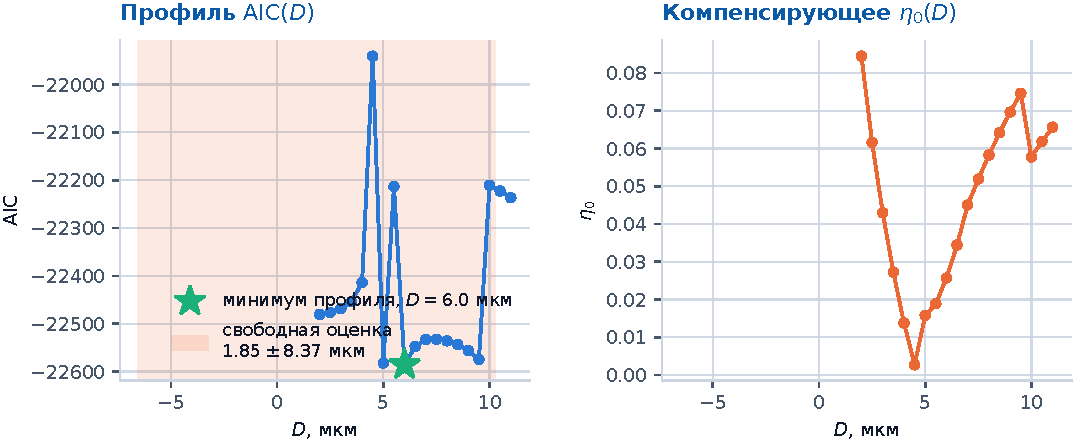
\includegraphics[width=\linewidth]{figures/fig09_profile.pdf}
  \caption{Слева: профиль $\AIC(\Deff)$ (та же кривая, что уже приводилась в §7 как иллюстрация
  множественных локальных минимумов, здесь~--- в контексте идентифицируемости). Справа: та же
  сетка значений $\Deff$, но по оси ординат~--- значение $\eta_0$, на которое переоптимизируются
  остальные параметры при каждом фиксированном $\Deff$: видно почти линейное компенсирующее
  движение~--- прямое графическое проявление вырождения, дополняющее число корреляции
  примера~\ref{subsec:degeneracy}.}
  \label{fig:profile}
\end{figure}

\begin{intuition}[: почему это не противоречие, а согласованная картина]
Свободная подгонка $1{,}85\pm8{,}37$~мкм и профильный минимум $6$~мкм не спорят друг с другом~---
они говорят одно и то же на разных языках. Огромная параболическая ошибка~--- симптом того, что
локальная (гауссова) аппроксимация вблизи найденной алгоритмом точки не годится глобально; профиль
честно показывает, что <<настоящий>> минимум может быть в стороне и не быть параболическим.
Обе картины согласны в главном: $\Deff$, оценённый свободно вместе с $\eta_0$, не является
надёжно измеренным числом.
\end{intuition}

% ---------------------------------------------------------------------
\subsection{Карта корреляций: с чем ещё конкурирует диаметр}
\label{subsec:corrmap}

Вырождение $\Deff\leftrightarrow\eta_0$~--- самое сильное, но не единственное. Полная карта
корреляций диаметра со всеми остальными параметрами опорной модели показывает, что диаметр
практически неотделим (корреляция по модулю $\gtrsim0{,}99$) от целой группы параметров,
отвечающих за амплитуду и фазу просачивания, и гораздо слабее связан с параметрами материала
(показатель рассеяния, коэффициент потерь) и офсетом угла.

\begin{figure}[t]
  \centering
  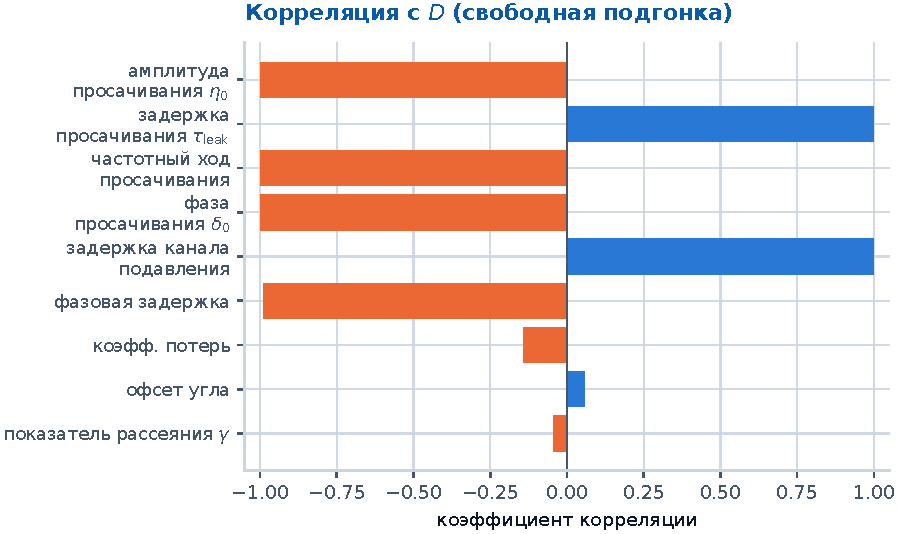
\includegraphics[width=0.82\linewidth]{figures/fig09_corrmap.pdf}
  \caption{Корреляция свободной оценки $\Deff$ со всеми остальными параметрами опорной модели при
  совместной подгонке (плотная решётка). Группа параметров просачивания практически неотличима от
  диаметра по модулю корреляции; параметры материала связаны с ним значительно слабее.}
  \label{fig:corrmap}
\end{figure}

\begin{intuition}[: практический вывод из формы карты]
Карта корреляций~--- готовый рецепт того, \emph{что именно} стоит фиксировать, а что можно
оставлять свободным. Параметр, слабо коррелирующий с диаметром (например, показатель рассеяния),
можно уверенно подгонять одновременно с ним. Параметр из группы с корреляцией, близкой к
единице, подгонять одновременно с диаметром бессмысленно~--- нужно зафиксировать один из пары на
независимо обоснованном значении, как это было сделано в §6--§7.
\end{intuition}

% ---------------------------------------------------------------------
\subsection{Бутстрап при вырождении: не эллипс, а «банан»}
\label{subsec:bootstrap-degenerate}

§7 предупреждал: бутстрап требует независимости пересемплируемых единиц. При вырождении
добавляется вторая ловушка, уже не про независимость данных, а про форму результата.

\begin{warning}[: линейная ошибка описывает вырождение только локально]
Формула~\eqref{eq:fisher} и эллипс ковариации~--- это локальное, линеаризованное описание. Когда
данные ограничивают не сам параметр, а нелинейную комбинацию нескольких параметров (как в
§\ref{subsec:degeneracy}), облако точек бутстрапа~--- повторных подгонок на пересемплированных
данных~--- часто вытягивается не в эллипс, а в изогнутую, «банановидную» полосу вдоль поверхности
уровня вырождения. Сообщать в этом случае только пару чисел (центр и симметричная ошибка)~---
терять как раз ту информацию о форме, ради которой бутстрап обычно и делают.
\end{warning}

\begin{intuition}[: как читать такой результат честно]
Правильный вывод из «банановидного» бутстрапа~--- не «параметр измерен плохо», а «данные измеряют
не этот параметр, а некоторую его комбинацию с соседним, и вот форма этой комбинации». Это
содержательный физический вывод, просто не в форме «значение $\pm$ ошибка», к которой хочется
свести любой результат.
\end{intuition}

% ---------------------------------------------------------------------
\subsection{Практический вывод: что и почему фиксировать}
\label{subsec:conclusion}

\begin{tcolorbox}[enhanced,colback=cS1!7,colframe=cS1,boxrule=0pt,leftrule=3pt,arc=1pt]
Собранный в этом параграфе аппарат объясняет решение, принятое ещё в §6--§7 без полного
обоснования: почему эффективный диаметр в опорной модели курса \term{фиксируется}, а не
подгоняется свободно. Свободная подгонка вместе с просачиванием измеряет не $\Deff$ и не
$\eta_0$ по отдельности, а их почти неразличимую комбинацию (§\ref{subsec:degeneracy}), причём
параболическая оценка ошибки в этой точке систематически вводит в заблуждение
(§\ref{subsec:profile}). Фиксация одного из вырожденной пары на независимо обоснованном значении
(например, физическом диаметре, где он доступен,~--- хотя, как показал §6, именно этот выбор
катастрофичен для качества подгонки, что само по себе физический результат) — единственный
способ получить осмысленную, а не иллюзорную оценку второго параметра.
\end{tcolorbox}

% ---------------------------------------------------------------------
\subsection{Типичные ошибки этого параграфа}

\begin{enumerate}[leftmargin=1.6em,itemsep=0.25em]
  \item Доверять параболической (фишеровской) оценке ошибки без проверки профильным
        правдоподобием, особенно вблизи известного или подозреваемого вырождения
        (§\ref{subsec:profile}).
  \item Интерпретировать огромную ошибку свободной оценки как «неточное измерение», а не как
        симптом вырождения, требующий фиксации одного из параметров.
  \item Сообщать результат бутстрапа при вырождении только как «значение $\pm$ ошибка», теряя
        форму облака точек, которая часто содержит больше физики, чем два числа
        (§\ref{subsec:bootstrap-degenerate}).
  \item Фиксировать параметр «для определённости», не проверив по карте корреляций, действительно
        ли он входит в сильно вырожденную группу (§\ref{subsec:corrmap}).
  \item Забыть, что вырождение~--- не патология конкретной подгонки, а прямое следствие
        ограниченного числа независимых чисел в измерении, о котором курс говорил ещё в §0 и §5:
        оно не лечится ни лучшим алгоритмом, ни большим числом итераций.
\end{enumerate}

\clearpage
